\chapter{Introduction}

%%%%%%%%%%%%%%%%%%
\section{Motivation}
%%%%%%%%%%%%%%%%%%
\null \quad \quad Many fields rely on graphical models as a framework for drawing inference on observational data, as they allow one to encode multivariate probability distributions. Inference on such models typically involves answering inference queries over a Bayesian network, that is, a directed acyclic graph (DAG) paired with an associated joint probability distribution. Computing inference queries is the process of reducing one probability distribution (typically via \textit{conditioning} and \textit{marginalizing}) into another simplified probability distribution from which we can draw samples, yielding a most probable configuration of the random variables involved. \newline
\null \quad \quad For instance, in the medical field, we may have observable data about a large number of patient symptoms (such as headache, cough, fever) and unobservable diseases (called \textit{latent} variables). We may wish to predict whether the patient has a specific disease or not given their observable symptoms. In this scenario, one would represent the data as a Bayesian network and query the model for the likelihood that a patient has the disease given the observable data. This amounts to evaluating the Bayesian network having observed the patient's symptoms, and sampling the resulting reduced probability distribution. This serves as the inference process, and allows for informed decision making. \newline 
\null \quad \quad The models discussed in this thesis have significant applications and adaptions in medicine~\cite{greenland1, greenland2, miller, pauker, shwe}, behavioral and social sciences~\cite{morgan, blalock}, and statistics~\cite{cox, lauritzen}. Furthermore, significant theoretical research has been done on graphical models themselves~\cite{verma, chickering, andersson}. An extensive survey of their genesis, development, and applications can be found in~\cite{pearlsurvey}. \newline
\null \quad \quad Naturally, especially as the use of statistical inference becomes increasingly widespread, it is in our best interest to explore methods for modeling and querying which allow us to do inference as quickly and efficiently as possible. In general, inference is a very expensive process; while there are state-of-the-art algorithms which approximate inference (such as MCMC-methods or variational inference~\cite{NUTS, varinf}), the speed of both these approximations and actual inference are limited. This thesis therefore take advantage of the Bayesian networks' property of non-identifiability, meaning that there can be several networks which encode the same probability distribution. Such networks are called \textit{Markov equivalent}. Markov equivalence informs us that a single inference query evaluated over structurally distinguishable Markov equivalent networks will always yield in statistically indistinguishable results. \newline 
\null \quad \quad We therefore explore the following question: given that the same probability distribution can be encoded in different Bayesian networks, \textbf{can it be computationally beneficial to change the representation of the probability distribution in order to answer a query more efficiently?} Additionally, can we use the same reasoning to answer a sequence of queries (for example, checking for multiple diseases at once) more efficiently?  \newline
\null \quad \quad Furthermore, in certain settings such as sampling, one does not evaluate an inference query over a probability distribution only once, but may instead wish to evaluate hundreds if not thousands of queries. Repeated evaluation of queries is a significant motivation for this work, as further justifies the overhead costs of transforming the networks.  \newline


%%%%%%%%%%%%%%%%%%
\section{Background}
%%%%%%%%%%%%%%%%%%
\null \quad \quad The family of models explored in this thesis are Bayesian networks over discrete probability distributions. The purpose of Bayesian networks is to encode information about vectors of random variables, namely the interdependencies satisfied by the vector's joint probability function. For example, consider a vector of three random binary variables $(X,Y,Z)$. Suppose that the values of $X$ and $Y$ depend on $Z$, but $X$ and $Y$ are independent from one another given $Z$. These dependencies can be encoded in the graph in Figure~\ref{fig:simpleencoding}, which is specified by its joint probability function.\newline
\begin{figure}[h!]
\begin{center}
\begin{tikzpicture}
\Vertex[x=-4.5, size=.5, color=white, label=$X$]{x}
\Vertex[x = -2.5, size=.5, color=white, label=$Y$]{y}
\Vertex[y = 1.5, x=-3.5 ,size=.5,color=white, label=$Z$]{z}
\Edge[Direct, distance=0.5](z)(x)
\Edge[Direct, distance=0.5](z)(y)
\Text[x=-3.5, y=-1]{$p(X,Y|Z) = p(X|Z) \cdot p(Y|Z)$}
\end{tikzpicture}
\end{center}
\caption{}
\label{fig:simpleencoding}
\end{figure}
\null \quad \quad In the case of the directed models we explore in this thesis, there is not necessarily a unique graph which satisfies the dependency constraints of the joint probability function. A random vector and its constraints may be represented by a variety of different graph structures which ultimately describe the same underlying probability distribution. To understand how the complexity of answering a query depends on graph structure, consider the two models in Figure~\ref{fig:introcomparison}.\newline
\begin{figure}[h!]
\begin{center}
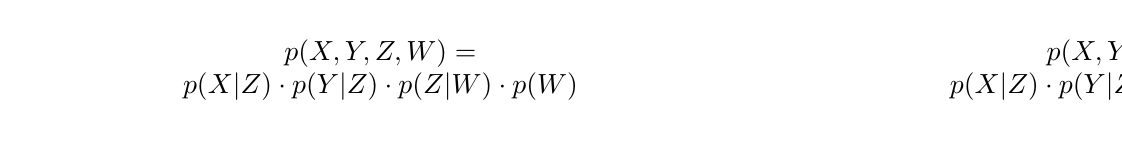
\begin{tikzpicture}
\Vertex[x=-3.5, y=3.5, color=white, label=$W$]{w}
\Vertex[x=-4.5, size=.5, color=white, label=$X$]{x}
\Vertex[x = -2.5, size=.5, color=white, label=$Y$]{y}
\Vertex[y = 1.5, x=-3.5 ,size=.5,color=white, label=$Z$]{z}
\Edge[Direct, distance=0.5](z)(x)
\Edge[Direct, distance=0.5](z)(y)
\Edge[Direct, distance=0.5](w)(z)
\Text[x=-3.5, y=-1]{$G_{1}$}
\node [below] at (-3.5, -2) {$\begin{array}{c} p(X,Y,Z,W) = \\  p(X|Z) \cdot p(Y|Z) \cdot p(Z|W) \cdot p(W)  \end{array}$};

\Vertex[x=4.5, y=3.5, color=white, label=$W$]{w}
\Vertex[x=3.5, size=.5, color=white, label=$X$]{x}
\Vertex[x = 5.5, size=.5, color=white, label=$Y$]{y}
\Vertex[y = 1.5, x=4.5 ,size=.5,color=white, label=$Z$]{z}
\Edge[Direct, distance=0.5](z)(x)
\Edge[Direct, distance=0.5](z)(y)
\Edge[Direct, distance=0.5](z)(w)
\Text[x=4.5, y= -1]{$G_{2}$}
\node [below] at (4.5, -2) {$\begin{array}{c} p(X,Y,Z,W) = \\  p(X|Z) \cdot p(Y|Z) \cdot p(W|Z) \cdot p(Z) \end{array}$};
\end{tikzpicture}
\end{center}
\caption{}
\label{fig:introcomparison}
\end{figure}
\null \quad \quad If we wish to answer a query about the random variable $Y$ in $G_{1}$, for instance the probability that $Y$ attains the value $y$, notated $p(Y=y)$, we must also compute the probabilities of each vertex it depends on either directly or indirectly: in this case, all of its \textbf{ancestors} (namely $Z$ and $W$) in addition to $Y$ itself. Alternatively, if we wish to answer a query $p(Y=y)$ on the graph $G_{2}$, we need only to compute $Z$ and $Y$. Then the number of variables which must be computed is reduced when we consider $G_{2}$ instead of $G_{1}$. The set of vertices a query depends on can somewhat vary depending on the query, but the motivation for transforming a network remains the same. \newline
\newpage
\null \quad \quad In a context where answering queries about a single vertex may require us to compute arbitrarily many other vertices in the graph, we seek an equivalent graphical representation of our probability distribution which minimizes the number of vertices that must be computed when answering a query. Further, we wish to explore the optimal sequence of transformations allowing us to answer a sequence of queries most efficiently. 

%%%%%%%%%%%%%%%%%%
\section{Goal}
%%%%%%%%%%%%%%%%%%
\null \quad \quad The central concept of this thesis is the exploitation of non-identifiability of Bayesian networks (Markov equivalence~\cite{verma}) for faster inference. Given that multiple Bayesian networks may encode the same probability distribution, the goals of our research are as follows: \newline
\null \quad \quad Given an inference query $q$ and a Bayesian network $B$ (which represents a single factorization of the probability distribution we wish to query), find a Markov equivalent Bayesian network $B'$ which minimizes the number of variables that must be evaluated to answer the query. The purpose of the minimization is to reduce the cost of evaluating $q$ in order to achieve faster inference, as well as evaluate the gained speedup versus the cost of transforming the representation. \newline
\null \quad \quad To achieve this, we first define the set of nodes which must be evaluated to answer $q$ over a given network $B$, notated $\Delta(B,q)$. Then, we search for a Markov equivalent Bayesian network $B'$ such that the size of $\Delta(B',q)$ is minimized. Finally, we compare the costs of computing the query over $B$ to the costs of computing the query over the minimized graph $B'$ plus the costs of identifying and transforming to $B'$. In short, the minimization problem is to determine the network $\Delta^{*}$ defined as
	$$\Delta^{*} = argmin_{B' \in [B]}|\Delta(B',q)|.$$
\null \quad \quad Subsequently, we consider how to identify optimal transformations for a known sequence of queries $\{q_{0}, q_{1}, ... q_{n}\}$ such that the overhead of transformation is most beneficial compared to the gained speedups by transforming.
%%%%%%%%%%%%%%%%%

\newpage
\section{Motivating Example}
%%%%%%%%%%%%%%%%%
\null \quad \quad The following example demonstrates how answering a query on one graph can be sped up by asking the same query over a Markov equivalent graph with a different structure. Consider the DAG in Figure~\ref{fig:motivatingdag}

\begin{figure}[h!]
\begin{center}
\begin{tikzpicture}
\Vertex[x=0, y=0, size=1,color=white, label=$X$]{x}
\Vertex[x=3.5,y=0, size=1, color=white, label=$Y$]{y}
\Vertex[x = 7, y=0, size=1, color=white, label=$Z$]{z}
\Edge[Direct, distance=0.5](x)(y)
\Edge[Direct, distance=0.5](y)(z)
\Text[x=3.5, y=-1.3]{$G_{1}$}
\end{tikzpicture}
\end{center}
\caption{}
\label{fig:motivatingdag}
\end{figure}

with conditional probabilities given by
\begin{align*}
	& p(X=1) = 0.2 			& \\
	& p(Y = 1 | X = 0) = 0.3		& p(Y = 1 | X = 1) = 0.4 \\ 
	& p(Z = 1 | Y = 0) = 0.1		& p(Z = 1 | Y = 1) = 0.9 
\end{align*}
and the joint probability
$$ p(X,Y,Z) = p(X) \cdot  p(Y|X) \cdot  p(Z|Y)$$
\null \quad \quad Here, if we wish to answer the query $p(Z|Y)$, our computation relies on all three random variables, since $Z$ relies on $Y$ and $Y$ relies on $X$. However, we can find a Markov equivalent graph in which we can answer the same query while relying on fewer random variables. Consider the DAG in Figure~\ref{fig:introdag}. 

\begin{figure}[h!]
\begin{center}
\begin{tikzpicture}
\Vertex[x=0, y=0, size=1,color=white, label=$X$]{x}
\Vertex[x=3.5,y=0, size=1, color=white, label=$Y$]{y}
\Vertex[x = 7, y=0, size=1, color=white, label=$Z$]{z}
\Edge[Direct, distance=0.5](y)(x)
\Edge[Direct, distance=0.5](y)(z)
\Text[x=3.5, y=-1.3]{$G_{2}$}
\end{tikzpicture}
\end{center}
\caption{}
\label{fig:introdag}
\end{figure}
\null \quad \quad We compute the conditional probabilities of $G_{2}$ and claim that the model can equivalently describe our joint probability distribution from $G_{1}$, and therefore be used to answer the query $p(Z|Y)$. We then observe how the structure of the new model affects our computation of the query. By applying Bayes' Theorem, which states that $p(A|B) = \frac{p(B|A)p(A)}{p(B)}$, we can compute
$$p(X|Y) = \frac{p(Y|X) \cdot p(X)}{p(Y)}  =  \frac{ p(Y|X) \cdot p(X) }{ \sum_{X} p(Y|X) \cdot p(X) }.$$

Using our pre-defined conditional probabilities,
\begin{align*}
	p(Y = 0) 	& \ \ = \ \ \sum_{X} p(Y = 0|X) \cdot p(X) \\ 
			& \ \ = \ \ 0.7 \cdot 0.8 + 0.6 \cdot 0.2 \\
			& \ \ = \ \ 0.56 + 0.12 \\
			& \ \ = \ \ 0.68
\end{align*}
and 
\begin{align*}
	p(Y = 1) 	& \ \ = \ \ \sum_{X} p(Y = 1|X) \cdot p(X) \\ 
			& \ \ = \ \ 0.3 \cdot 0.8 + 0.4 \cdot 0.2 \\
			& \ \ = \ \ 0.24 + 0.08 \\
			& \ \ = \ \ 0.32.
\end{align*}

which allow us to compute 
$$
	p(X = 1 | Y = 0) \ \ = \ \ \frac{p(Y = 0 | X=1) \cdot p(X=1)}{p(Y=0)} \ \ = \ \ \frac{0.6 \cdot 0.2}{0.68} \ \ \approx 0.176
$$

and
$$
	p(X = 1 | Y = 1) \ \  = \ \  \frac{p(Y=1 | X=1) \cdot p(X=1)}{p(Y=1)} \ \ = \ \ \frac{0.4 \cdot 0.2}{0.32} \ \ = 0.25.
$$

\null \quad \quad Then, since $X$ and $Y$ do not depend on $Z$, the conditional probability of $Z$ remains unchanged. Therefore, model $G_{2}$ is an equivalent model to $G_{1}$. If we answer the query $p(Z|Y)$ on model $G_{2}$, we do not need to consider $X$, since $Y$ (and consequently $Z$) no longer depends on $X$. \\
\null \quad \quad Through this example, we see that it may be possible to find an equivalent graph to our original model, and to use the new graph structure to answer certain queries more efficiently. It is important to note that the efficiency of the new model for answering a query depends on the content of our query (as opposed to an arbitrary query). 


%%%%%%%%%%%%%%%%%%
\section{Related work}
%%%%%%%%%%%%%%%%%%
\null \quad \quad Significant work has been done on individual aspects of the subject, though this thesis pioneers in using them together for fast inference. Verma and Pearl\cite{verma} give a framework for understanding how the same probability distribution can be encoded into two distinct graphs and present a simplified criterion for when two graphs describe indistinguishable distributions. Lucas and Flesch\cite{flesch} present a survey-style overview of Markov Equivalent graph structures, reduction of graph structures to simplified representations of equivalent distributions, as well as providing a strong background of relevant graph theory and probability preliminaries. Chickering\cite{chickering} explores parameters of equivalent networks, presents a procedure for altering graphs without changing the described probability distribution, and quantifies the complexity of several such manipulations. Andersson \textit{et. al.}\cite{andersson} make similar headway by exploring reductions of graphs to representative form, as well as describing procedures by which one can alter the structure. \newline 
\null \quad \quad Adjacently, Schachter\cite{schachter} confronts the same goal of faster inference of queries using a different method in a modified setting. His task focuses on eliminating unnecessary nodes from the computations directly, rather than by reversing edges. 

%%%%%%%%%%%%%%%%%%
\section{Outline}
%%%%%%%%%%%%%%%%%%
\null \quad \quad In Chapter 2, we introduce preliminary concepts from graph theory and Bayesian statistics to robustly define our models and to aid our understanding of graph manipulations and the process of querying over a graph. Chapter 3 details the problem and proposed querying method, then aims to quantify the computational costs of answering an arbitrary query over a graph by this method. Chapter 4 builds context for understanding Markov equivalence between graphs. In Chapter 5, we examine the circumstances under which Markov equivalence can be utilized to answer a query more efficiently, and then quantify the computational costs of finding a suitable Markov equivalent graph for faster inference. Finally, in Chapter 6, we compare the quantities explored in Chapters 3 and 5 to determine whether our proposed algorithm indeed increases inference speed, and if so, where it is effective. Additionally, we explore the usefulness of graph transformation in the context of sequences of queries rather than an individual query. Finally, in Chapter 7, we present the conclusions, implications, and possible future work. 